\documentclass{article}
\usepackage[utf8]{inputenc}
\usepackage{mathtools}
\usepackage{amssymb}
\usepackage{graphicx}
\usepackage{caption}
\usepackage{float}
\usepackage{amsthm}

\newtheorem{preuve}{Preuve}


\font\myfont=cmr12 at 30pt
\title{{\myfont Modèle de battement du cœur}}
\author{Clément GILLI, Louis-Alexis PENELOUX }
\date{Novembre 2022}

\begin{document}

\maketitle

\section{Résumé}

\[\]

On étudie les phénomènes électriques accompagnant le battement cardiaque, ou
plus précisément, le comportement électrique d’une cellule cardiaque, en essayant de mettre en
évidence des propriétés mathématiques significatives. On propose un modèle analogique de la contraction
d’une cellule du cœur comme exemple d’un phénomène oscillatoire avec relaxation. Ce
modèle conduit à l’équation de Van der Pol, dont on étudie des propriétés qualitatives analytiquement ou bien numériquement.
On essaye d'obtenir un modèle le plus fidèle possible aux observations.

\section{Modèle du battement du cœur et oscillations avec relaxation}

\[\]

On veut modéliser les battements du cœur. Depuis la fin du dix-neuvième siècle, on sait que l’activité cardiaque est associée à la production d’une quantité de courant électrique.
D'après les observations physiques, on sait que le phénomène de battement de coeurs fait partie des systèmes naturels auto-excités, c'est-à-dire qu'il sort lui même de son état de repos, dont on remarque des oscillations avec relaxation. Un exemple de système auto-excité est donné par les circuits éléctriques  RLC. On décrit rapidement ce modèle, puis on montrera qu'un habile choix de $\varepsilon$ peux alors ajouter des oscillations avec relaxation à notre système.


\begin{equation}
   \left\{
   \begin{aligned}
        x'(t) &= \varepsilon (y(t) - f(x(t)))\\   
        y'(t) &= -x(t)\\
   \end{aligned}
   \right.
\end{equation}
avec $\varepsilon \in \mathbb{R}$


Si on choisit \(f(x) = \frac{1}{3} x^3 - x\), le système (1) est appelé système de Van der Pol. En dérivant $x'$ et en remplaçant $y'$ par son expression donnée dans le système, on obtient l'équation :

\begin{equation}
    \frac{1}{\varepsilon} x''(t) + (x(t)^2 -1)x'(t) + x(t) = 0
\end{equation}

On peut montrer que (1) et (2) sont bien équivalent, $i.e.$ toute solution de (1) est solution de (2), et réciproquement.

En effet, (1) s'écrit
\begin{equation*}
    \left\{
    \begin{aligned}
        x'(t) &= \varepsilon (y(t) - \frac{1}{3} x(t)^3 + x(t)) \\   
        y'(t) &= -x(t)\\
   \end{aligned}
   \right.
\end{equation*}
dont on dérive la première ligne et remplace \(y'(t) \) par \( -x(t) \) pour obtenir le résultat voulu.
Réciproquement, supposons que \(x\) respecte (2), et que de plus elle admette une primitive sur $\mathbb{R}$. Posons alors $y$ l'unique primitive de $-x$ valant $\frac{x'(0)}{\varepsilon} 
+ \frac{x(0)^3}{3} - x(0)$ en $0$.
On a $y'(t) = -x(t)$, donc en injectant dans (2),

\begin{equation*}
    x''(t) = \varepsilon (x'(t) - x'(t)x(t)^2 + y'(t)) \\
\end{equation*}
En intégrant ces deux quantités, on obtient
\begin{equation*}
    x'(t) = \varepsilon (x(t) - \frac{x(t)^3}{3} + y(t)) + C \\
\end{equation*}
avec $C$ la constante d'intégration. En évaluant en 0, on obtient bien $C = 0$. La première ligne est respectée et l'équivalence est montrée.

\medskip

On remarque qu'on a ajouté une perturbation au coefficient de $x'$ car sinon on aurait une solution sinusoïdale, ce qui ne va pas avec le modèle souhaité. En effet, si le coefficient de $x'$ est nul, et si on pose $\varepsilon = 1$, (les autre cas étant tout aussi simples), l'équation s'écrit :

\begin{equation*}
    x''(t) + x(t) = 0
\end{equation*}

On peut facilement résoudre cette équation, et on obtient :
\[ x(t) = \lambda \cos t + \mu \sin t\]
avec $\lambda ,\mu \in \mathbb{R}$

À partir de là, on peut primitiver $x$ pour trouver $y$ à partir de (1) :

\[ y(t) = -\lambda \sin t + \mu \cos t\]

On remarque notamment que pour tout $t$,  $x(t)^2 + y(t)^2 = 1$. La solution a une allure de cercle : on peut tracer $y(t)$ en fonction de $x(t)$ (on pose $\lambda = \mu = 1$)  $(Figure$ 1$)$ 

\begin{figure}[H]
\centering
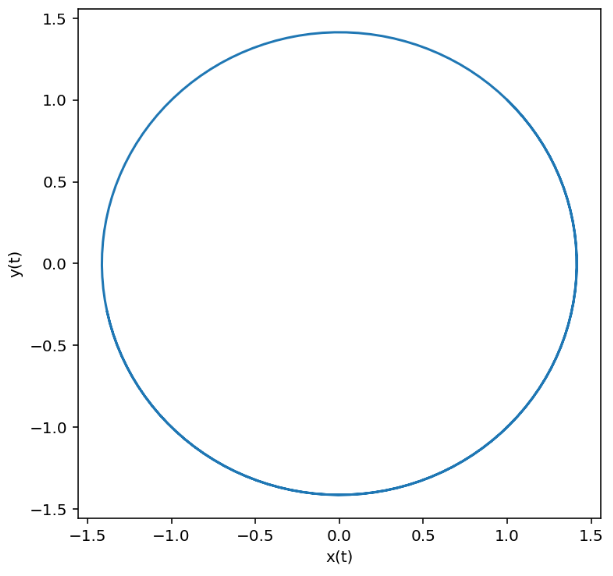
\includegraphics[scale=0.5]{../images/plot_circ.png}
\caption{Graphe de $y(t)$ en fonction de $x(t)$}
\end{figure}

Ce n'est pas satisfaisant. On est obligé de rajouter cette perturbation pour construire un modèle cohérent avec les données physiques.

\section{Étude qualitative de l’équation de Van der Pol}

\[\]

Dans cette section, on décrit brievement quelques propriétés du système de Van der Pol, avec $\varepsilon = 1$ fixé :

\begin{equation}
    \left\{
    \begin{aligned}
        x'(t) &= y(t) - \frac{1}{3} x(t)^3 + x(t) \\   
        y'(t) &= -x(t)\\
   \end{aligned}
   \right.
\end{equation}

\begin{enumerate}
    \item Le seul équilibre de (3) est $(0, 0)$ et c’est une source
    \item Le problème de Cauchy pour (3) a une unique solution pour toute donnée initiale
    \item Les trajectoires tournent dans le sens des aiguilles d’une montre autour de l’origine
    \item Il y a une unique solution périodique non triviale que l’on appelle $\gamma$ 
    \item Les autres trajectoires (non triviales) s’approchent de $\gamma$ en tournant
\end{enumerate}

\medskip

\begin{preuve}

\medskip

Le système est en équilibre si et seulement si $x$ et $y$ sont constantes, $i.e.$ 
si et seulement si $x'$ et $y'$ sont nulles, $i.e.$ 
si et seulement si $ \forall t,$ $x(t)=0$ et $y(t)=0$. Donc le seul équilibre de (3) est $(0,0)$ (En effet, c'est l'unique solution constante d'après le théorème de Cauchy-Lipschitz).
\\À présent, on étudie le comportement du système (3) linéarisé pour voir le comportement des points d'équilibre, $i.e. (0,0)$ ici :

\begin{equation*}
    \left\{
    \begin{aligned}
        x'(t) &= y(t) + x(t) \\   
        y'(t) &= -x(t)\\
   \end{aligned}
   \right.
\end{equation*}

On pose $u =\begin{pmatrix}x(t)\\y(t)\end{pmatrix}$ et $A=\begin{pmatrix}1 & 1\\-1 & 0\end{pmatrix}$. On a donc $u' = Au$
\smallskip
\\Or $P_A(X)=\begin{vmatrix}1-X & 1\\-1 & -X\end{vmatrix} = X^2-X+1$
\smallskip
\\Donc $Sp_\mathbb{C}(A) = \{ \frac{1}{2} - i \frac{\sqrt{3}}{2}, \frac{1}{2} + i \frac{\sqrt{3}}{2} \} = \{z_1,z_2\}$
\smallskip
\\On a donc $Re(z_1)>0$ et $Re(z_2)>0$, ainsi que $z_1 = \bar{z_2} \implies (0,0)$ est une source ! $\square$   

\end{preuve}

\begin{preuve}
On peut réécrire le système (3) sous forme de problème de Cauchy $X' = f(t,X) $ avec $X=(x(t),y(t))$
et $f:\mathbb{R}^3 \to \mathbb{R}^2$ définie par

\begin{equation}
    f(t,(x,y)) = (y - \frac{1}{3} x^3 + x,-x)
\end{equation}

Or $f$ est clairement $\mathcal{C}^1$, donc elle est lipzitchienne par rapport à sa seconde variable, ici $(x,y)$.
\\Ainsi, d'après le théorème de Cauchy-Lipschitz, (3) a une unique solution pour toute donnée initiale. $\square$
\end{preuve}

\begin{preuve}

Cette fois ci, on va prouver cette propriété numériquement. 
On a donc résolu numériquement le système (3), puis tracé différentes solutions à partir de conditions initiales $(x_0,y_0)$ différentes $(Figure$ 2$)$.
On a également tracé le champs de vecteur associé. On constate que peu importe le point $(x_0,y_0)$ de départ, la courbe finit toujours par tourner autour de l'origine dans le sens des aiguilles d'une montre.
Le champs de vecteur permet de bien visualiser le sens de rotation. $\square$

\begin{figure}[!h]
\centering
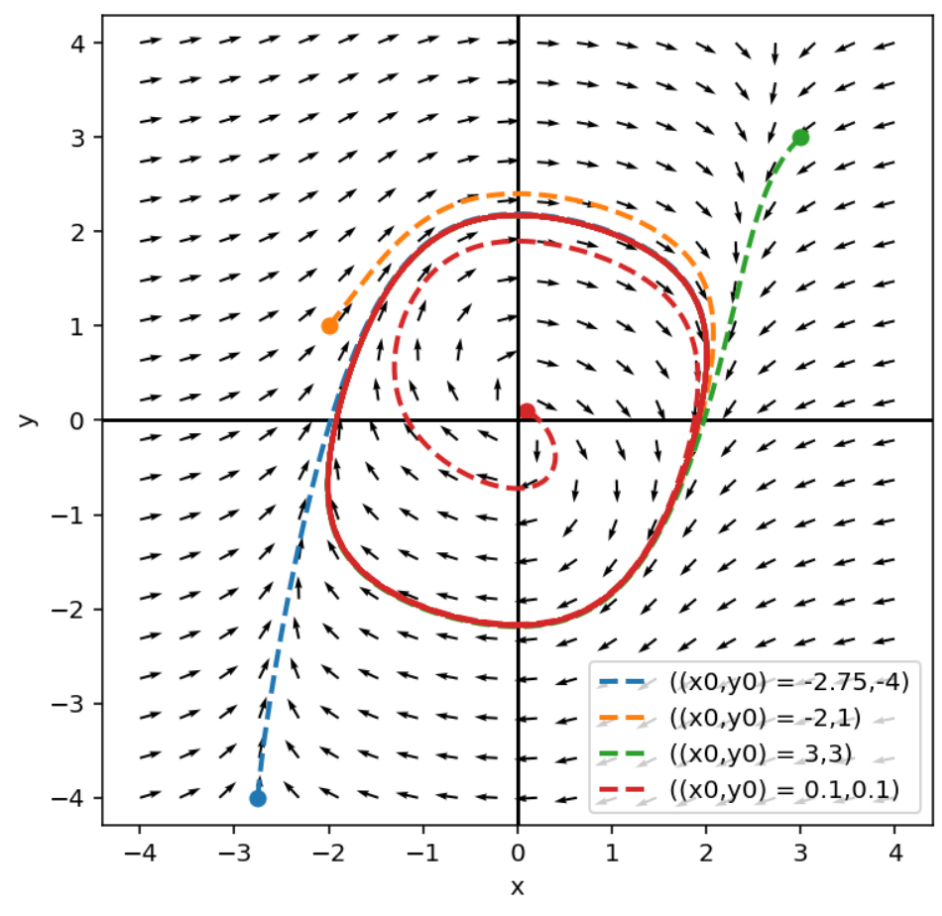
\includegraphics[scale=0.4]{../images/plot_solh.png}
\caption{Diagramme des phases}
\end{figure}

\end{preuve}

On admettra la preuve des autres propriétés. On peut cependant utiliser le schéma de Runge Kutta pour montrer les résultats attendus $(Figure$ 3$)$.
On en profite pour remarquer la présence d'une unique solution périodique $\gamma$ non sinusoïdale.
Pour toutes données initiales autres que la source $(0,0)$, l'allure des solutions se rapprochent de $\gamma$.

\begin{figure}[!h]
\centering
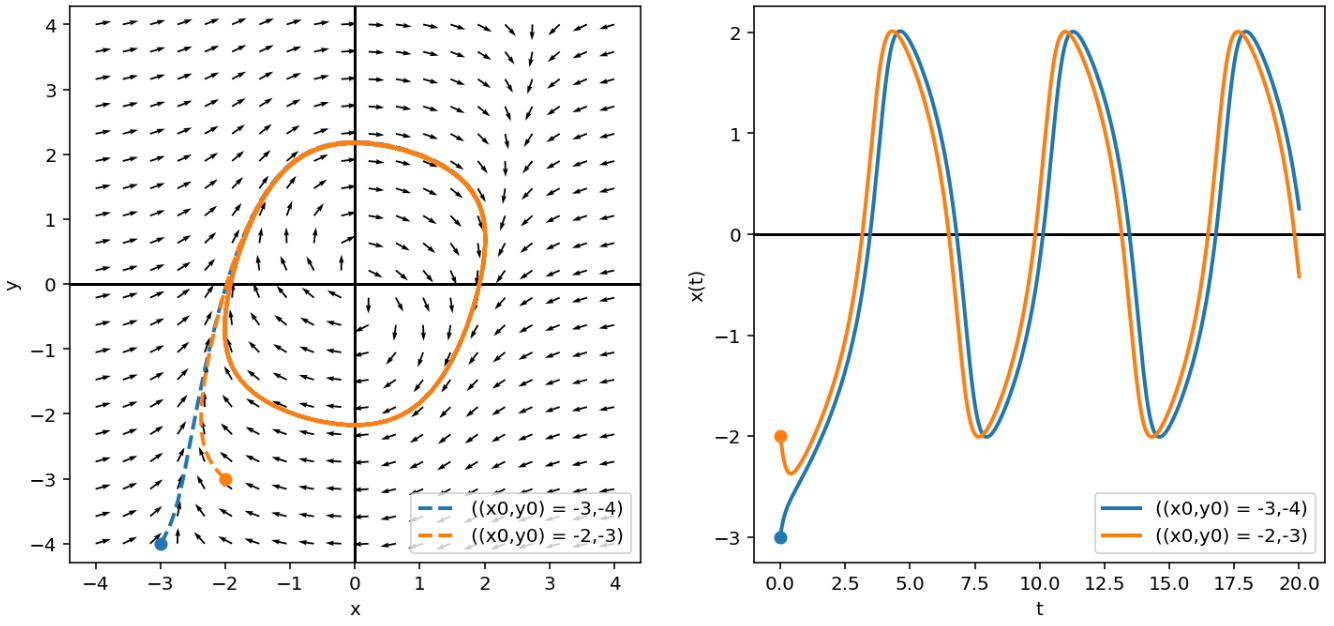
\includegraphics[scale=0.4]{../images/dphase.png}
\caption{Diagramme des phases et intensité du courant en fonction du temps}
\end{figure}

\newpage
\section{Choix du paramètre $\varepsilon$}

\[\]

On essaye de choisir $\varepsilon$ pour obtenir un comportement oscillatoire avec relaxation, avec pour
but principal d’obtenir des oscillations sensiblement non sinusoïdales. Pour cela, on remarque
que si $0 <\varepsilon < 1$, on obtient numériquement des courbes presque sinusoïdales. On n'étudiera pas le cas
$\varepsilon \leq 0$.
On est donc amené à considérer des valeurs positives et élevées du paramètre $\varepsilon$. 
Par exemple, pour $\varepsilon = 100$, on a le comportement décrit par la $Figure$ 4.
Dans le diagramme des phases de la $Figure$ 4, on peut aussi remarquer que quand $\varepsilon$ est grand,
certaines parties de la trajectoires et de la courbe $y = f (x)$ sont très proches l’une de l’autre (avec un léger déphasage). On va donc choisir $\varepsilon$ positif et "grand" (dans les exemples, on gardera
$\varepsilon$ = 100).

\begin{figure}[!h]
    \centering
    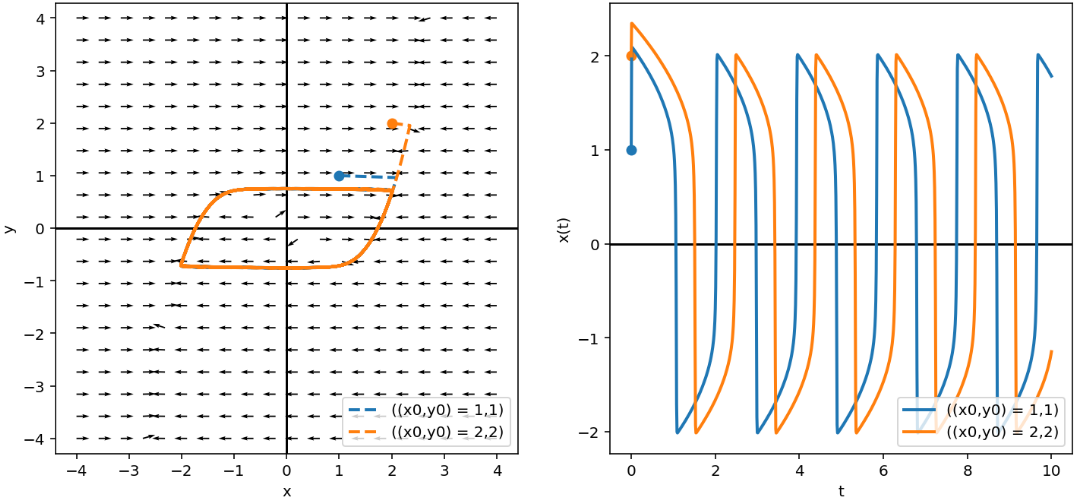
\includegraphics[scale=0.4]{../images/epsilon_choice.png}
    \captionsetup{justification=centering,margin=2cm}
    \caption{Diagramme des phases et intensité du courant en fonction du temps avec $\varepsilon = 100$}
\end{figure}

\section{Période et amplitude asymptotique}

\[\]

On veut maintenant estimer la période fondamentale $T$ de la solution. Pour cela, on remarque qu'analytiquement c'est assez complexe, c'est pourquoi on décide de l'estimer numériquement.
L'algorithme est assez simple en pratique: On cherche le point où la valeur de l'ordonnée est maximale (une fois que la solution s'est stabilisée) puis on cherche le prochain point où l'ordonnée est maximale.
En faisant la différence des abscisses, on obtient une approximation de la période ($Figure$ 5).
En faisant tendre $\varepsilon$ vers $+\infty $, le résultat analtyique (admis ici) nous dit que $\lim_{\varepsilon \to \infty} T = 3 - 2\ln 2 \simeq 1.61$.
Avec notre algorithme assez naïf, on arrive à trouver $T \simeq 1.66$ pour $\varepsilon$ assez grand.

\begin{figure}[!h]
    \centering
    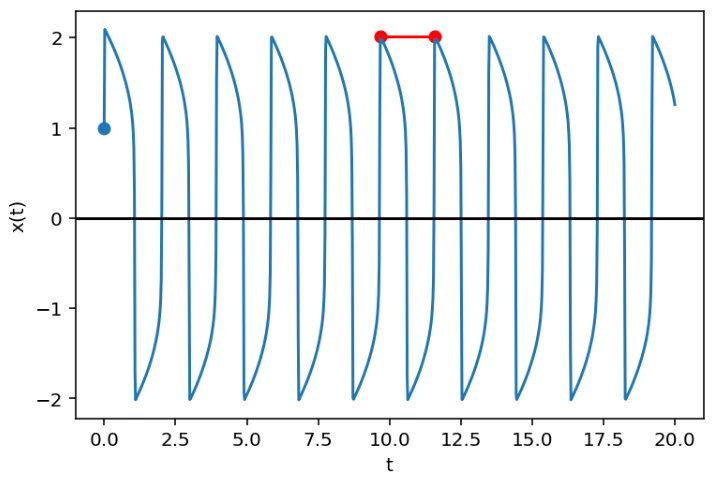
\includegraphics[scale=0.5]{../images/periode.png}
    \captionsetup{justification=centering,margin=2cm}
    \caption{Intensité du courant en fonction du temps avec $\varepsilon = 100$. La période estimée est $T \simeq 1.9$}
\end{figure}

\section{Un autre modèle : $f$ linéaire}

\[\]

Lorsqu'on choisit f linéaire dans le système $(1)$, la solution n'est pas périodique.
En effet, on voit qu'elle s'écarte très vite de la source ($Figure$ 6).
Pour tout autre degré que 1 et 3 pour le $f$, les observations numériques sont chaotiques, ce qui laisse supposer que le modèle n'est pas viable. 

\begin{figure}[H]
    \centering
    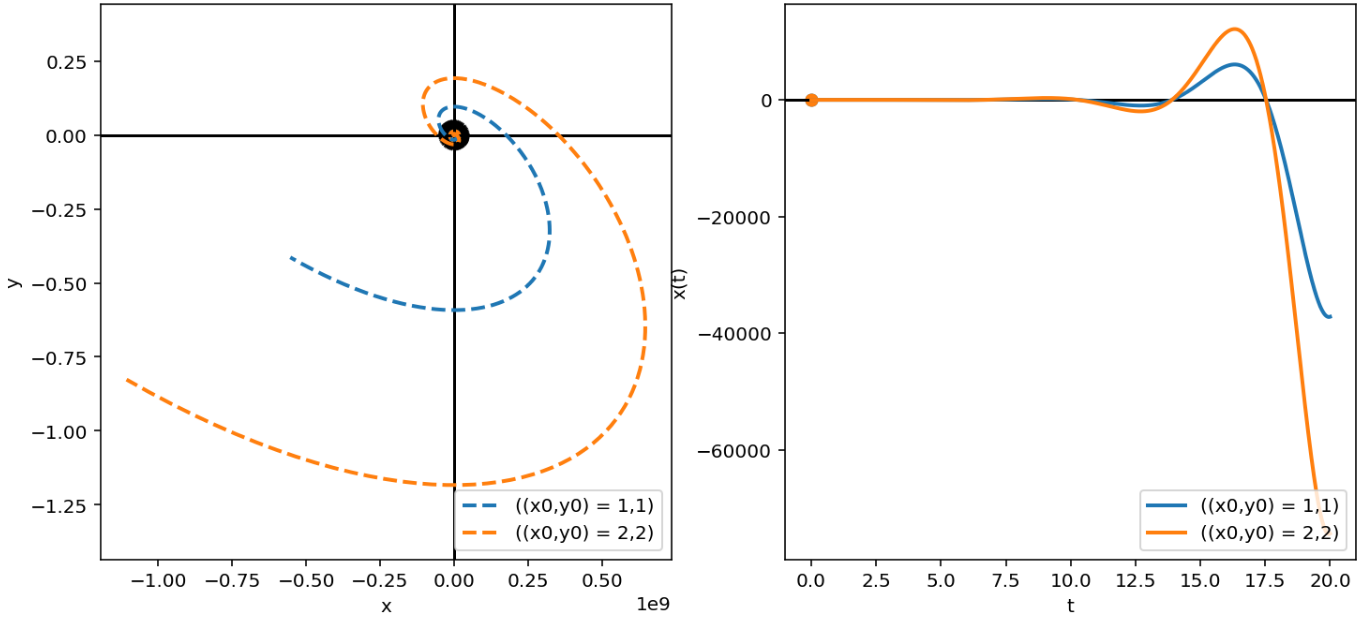
\includegraphics[scale=0.3]{../images/diff_f.png}
    \captionsetup{justification=centering,margin=2cm}
    \caption{Diagramme des phases et intensité du courant en fonction du temps avec $f(x) = x$ }
\end{figure}

\section{Conclusion}

\[\]

D'après les résultats démontrés, ainsi que ceux observés numériquement, on obtient, pour 
\(f(x) = \frac{1}{3} x^3 - x\), une solution qui tend rapidement vers une solution périodique.

\smallskip

La donnée initiale correspond a une impulsion envoyé au système cardique (similaire à un électrochoc).

\smallskip

Pour que la solution limite soit la plus proche possible des observations, on joue sur le paramètre $\varepsilon$.
On observe qu'il faut qu'il soit assez important.

\smallskip

Si $f$ est polynomiale, on remarque que seul un polynome de degré 3 semble convenir.
Pour affiner le système, il faudrait alors considérer une fonction $f$ "assez proche" d'une fonction 
polynomiale de degré 3.

\end{document}